\chapter{Details on Natural Gradient Descent with CIQ-Based SVGP}
\label{app:ngd}

\section{Additional SVGP Results}

\begin{figure}[ht!]
  \centering
  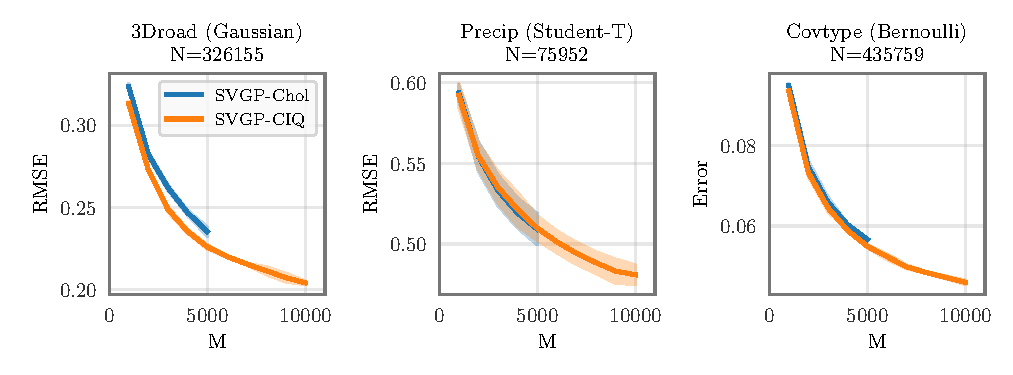
\includegraphics[width=\linewidth]{figures/variational_error.pdf}
  \caption[RMSE comparison of Cholesky-whitened vs CIQ-whitened SVGP models.]{
    RMSE comparison of Cholesky-whitened vs CIQ-whitened SVGP models.
    {\bf Left:} 3DRoad dataset ($N=326155, D=2$, Gaussian likelihood).
    {\bf Middle:} Precipitation dataset ($N=75952, D=3$, Student-T likelihood).
    {\bf Right:} CoverType dataset ($N=435759, D=54$, Bernoulli likelihood).
    NLL improves with more inducing points ($M$), and Cholesky and CIQ models have similar performance.
    However CIQ scales to larger values of $M$.
  }
  \label{fig:variational_error}
\end{figure}
